\subsection{Teilversuch 5: Kristallpolarisation an einem Kalkspat}

	\subsubsection*{Methoden}
		
		\begin{figure}[ht]
			\centering
			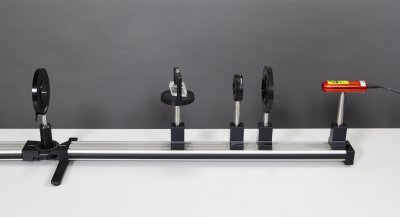
\includegraphics[width=\textwidth]{bilder/Kalkspat.png}
			\caption{Aufbau des letzten Teilversuches\cite{WWU}}
			\label{fig:Kalkspat}	
		\end{figure}
		Abb. \ref{fig:Kalkspat} stellt den Aufbau für den letzten Teilversuch dar.
		Hier werden zwischen die Polarisatoren das $\lambda/2$-Plättchen und der Kalkspat gesetzt.
		Die Photodiode soll bei diesem Versuch nicht verwendet werden.
		Stattdessen soll ein Schirm hinter dem zweiten Polarisator stehen, auf dem die Intensität des Laserlichts beobachtet und diskutiert werden soll.
		
	\subsubsection*{Durchführung}
	
		Nach dem Einsetzen der Versuchsmaterialien und folgender Inbetriebnahme des Lasers ließen sich vier Lichtpunkte auf dem Schirm ausmachen.
		Drehen des $\lambda/2$-Plättchens führte dazu, dass jeweils zwei der Lichtpunkte verschwanden, nach weiteren \SI{45+-0,4}{\degree} wieder auftauchten und dafür die anderen beiden an Intensität verloren.
		Bei dem Drehen des zweiten Polarisators wurde das gleiche, nur mit anderen Paaren der Punkte, bei \SI{90+-0,4}{\degree} beobachtet.
		Waren es bei dem $\lambda/2$-Plättchens die Punktpaare (1,2) und (3,4), so waren es beim dem Polarisastor die Paare (1,4) und (2,3).
		Für den Fall, dass beide so gedreht waren, dass je ein Paar verschwindet, war nur einer der vier Lichtpunkte sichtbar.
		
	\subsubsection*{Diskussion}
	
		Die Beobachteten Verhältnisse lassen sich auf die Polarisation an Kristallen zurückführen.
		Bei dem Strahlengang durch den Kristall, wird der Strahl in zwei Teile geteilt.
		Einerseits in den "ordentlichen" Strahl, welcher sich gemäß dem Snellius'schen Brechungsgesetz verhält und mit dem Brechungsindex $n_1$ in dem Kristall gebrochen wird, sowie andererseits dem "außerordentlichen" Strahl, welcher um einen anderen Winkel durch den Brechungsindex $n_2$ gebrochen wird.
		Die Strahlen sind nach austritt aus dem Kristall orthogonal zueinander polarisiert.
		Hier soll der parallele und senkrechte Anteil auf die Kristallstruktur bezogen sein.
		
		Trifft linear polarisiertes Licht mit einem senkrechten und einem parallelen Anteil auf den Kristall, so werden beide jeweils in einen ordentlichen und einen außerordentliche Strahl gebrochen.
		Daher lassen sich vier Lichtpunkte auf dem Schirm erkennen.
		Wird das $\lambda/2$-Plättchen so gedreht, dass der senkrechte Anteil gerade gleich null wird, das Eingangslicht also parallel polarisiert ist, so wird nur der parallele Anteil in zwei Strahlen geteilt und es sind nur zwei Lichtflecke auf dem Schirm erkennbar.
		Ebenso sind die anderen beiden Lichtflecken erkennbar, wenn das Eingangslicht gerade senkrecht polarisiert ist.
		Dass nach \SI{45+-0,4}{\degree} die Polarisation jeweils wechselt ist dem zweiten Teilversuch zu entnehmen.
		Analog mit dem zweiten Polarisator nach \SI{90+-0,4}{\degree}.
		Für den Fall, dass nach dem Drehen des $\lambda/2$-Plättchens nur noch zwei Lichtpunkte zu erkennen sind, lässt sich durch Drehen des zweiten Polarisators einer der beiden Strahlen auslöschen, indem diese gerade senkrecht aufeinander stehen.
		Auch hier wird dann nur der parallele bzw. senkrechte polarisierte Anteil des Lichtstrahls hinter dem Kristall durchgelassen.
		Somit lässt sich dieses Phänomen der vier unterschiedlich reagierenden Lichtpunkte erklären.